\chapter{Special Cases and Restrictions}
\label{chapter:special}

Having proven that \probBook is a hard problem in the previous section,
we now turn to some special instances or variations on \probBook and
either show how they can be solved efficiently or why they remain hard.
This section is the main contribution of this thesis.

One topic we are interested in is how embeddability depends
on the connectivity of the pages. Thus, we deal with both extreme
cases with regards to connectivity in the first two sections: The pages
can either all be connected~(\myref{section:connected}), or ``maximally
disconnected'' without isolated vertices~(\myref{section:matchings}), \ie consisting of perfect disjoint matchings.

We show that the connected case---quite surprisingly---admits a solution
in linear time.
For each page we get a \PQ-tree (see \myref{def:pq}) that stands for the
possible orders of the vertices in a page embedding of this single page.
The solution intersects these sets of orders to decide embeddability. 

In contrast, we are unable to provide an efficient algorithm if the edges of each
page form perfect disjoint matchings. We only manage to prove for this
case that an embeddable graph must be bipartite. Furthermore, we derive---by hand and using a computer---positive bipartite instances and the smallest bipartite counterexamples for all numbers of pages with the
exception of three pages. For three pages we are able to get a smallest counterexample
when two of the matchings form a cycle.

Another interesting restriction we make in \myref{section:trees} is to allow the order of the 
vertices on the spine to only come from the
permutations represented by a fixed \PQ-tree. We present a quadratic time algorithm
for solving the book embedding problem with this restriction if we only allow \Q-trees.
Angelini et.\,al.~\cite{angelini11} showed that a similar restriction is important by reducing \SEFECON~(see page~\pageref{prob:sefecon}) to a book embedding problem
with 2~pages constrained by a \PT-tree.

Finally, in \myref{section:multi_spine} we give a related 
variation on the book embedding problem. We now allow multiple spines~(parallel lines) in the plane
and associate every vertex with a spine the vertex has to be drawn on. 
Additionally, we demand that edges are drawn between consecutive spines, above the
topmost spine or below the bottommost spine. We show that this variation is equivalent to
a special case of the 2-page book embedding problem where the vertex order is constrained
by a \PT-tree, \ie it is indeed related to the problem
of \myref{section:trees}.

While the results we present are mostly independent of each other and small, they
still provide significant insight into the book embedding problem and
\myref{section:trees} is a step towards solving \prob{sefe}. 

\section{Connected pages}

\begin{frame}[fragile]{Linear-time decision}

\begin{theorem}
\probBook with connected pages can be solved in $\OO(n)$~time.
\end{theorem}

\begin{overprint}
\onslide<1>
\begin{itemize}
\item Construct \PQ-trees $T_i$ on~$V$ representing valid orders of individual pages
$(V,E_i)$
\begin{figure}
\centering
\resizebox{0.8\textwidth}{!}{
\begin{tikzpicture}
\path[use as bounding box] (-2,2) rectangle (8,-2.5);

\tikzstyle{every node}+=[minimum size=0.5cm,thick]
\tikzstyle{every path}+=[thick]

\node[] (a) {$a$};
\node[right of=a] (b) {$b$};
\node[below of=b] (c) {$c$};
\node[left of=c] (d) {$d$};

\draw (a) edge (b) 
      (b) edge (c) 
      (c) edge (d) 
      (d) edge (a);
\end{tikzpicture}}
\end{figure}
\end{itemize}

\onslide<2>

\begin{itemize}
\item Construct \PQ-trees $T_i$ on~$V$ representing valid orders of individual pages
$(V,E_i)$
\begin{figure}
\centering
\resizebox{0.8\textwidth}{!}{
\begin{tikzpicture}
\path[use as bounding box] (-2,2) rectangle (8,-2.5);

\tikzstyle{every node}+=[minimum size=0.5cm,thick]
\tikzstyle{every path}+=[thick]

\node[] (a) {$a$};
\node[right of=a] (b) {$b$};
\node[below of=b] (c) {$c$};
\node[left of=c] (d) {$d$};
\node[left of=a, above of=a] (r) {$r$};

\draw (a) edge (b) 
      (b) edge (c) 
      (c) edge (d) 
      (d) edge (a);
\draw[dashed] (r) edge (a)
              (r) edge (b)
              (r) edge (d)
              (r) edge[out=270, in=270, min distance=6em] (c);

% PQ-tree
\begin{scope}[xshift=5cm]
\node[draw,rectangle,minimum size=.2cm] {}
   child {node {$a$}}
   child {node {$b$}}
   child {node {$c$}}
   child {node {$d$}};
\end{scope}
\end{tikzpicture}}
\end{figure}
\end{itemize}

\onslide<3>
\begin{itemize}
\item Construct \PQ-trees $T_i$ on~$V$ representing valid orders of individual pages
$(V,E_i)$
\item Intersect the $T_i$ [Booth, 1975]
\item[$\rightarrow$] Resulting \PQ-tree~$T$ represents valid book orders
\end{itemize}
\end{overprint}

\end{frame}

\section{Perfect Matchings}\label{section:matchings}

A diametrically opposed simplification to \myref{section:connected} is to take disjoint
perfect matchings as graphs on the pages since matchings are---in a sense---the most disconnected graphs apart
from isolated vertices.
That is, we least expect to be able to adapt the result for connected graphs to this new setting.
Note that this is only possible for an even number of vertices and remember that we
have shown the \NP-completeness when taking (not necessarily perfect) matchings as pages in \myref{section:np-complete}.

\newProb{\probMatching}
{Disjoint perfect matchings $E_1,\dotsc, E_k$ on a vertex
set $V$.}{Is there a book embedding of $(V, E_1),\dotsc, (V, E_k)$?}

In this section we first show that an embeddable instance of \probMatching has to be
\emph{bipartite}, \ie the \emph{union graph}~$(V, E_1\cup\dotsb\cup E_k)$ must be bipartite. Then we prove that the problem does not become trivial for any number~$k$ of pages
by providing positive and negative bipartite instances.
For all~$k$ we get a partition of $K_{k,k}$, the complete bipartite graph with $k$~left and $k$~right vertices, as smallest (vertex-minimal) positive bipartite instance and
for $k > 3$ we get another partition of~$K_{k,k}$ as smallest negative bipartite instance.
We show this by hand in \myref{subsec:four}. Getting a smallest bipartite counterexample
for~$k = 3$ is significantly more difficult and we have to resort to using computer assistance in
\myref{subsec:three}. Even with the computer we only manage to find a smallest
bipartite counterexample when two of the matchings are required to form a cycle.

\begin{figure}[\placement]\centering
    \includegraphics[scale=2.0]{figures/t_k4}
    \caption[$K_4$ is not embeddable]{A non-embeddable partition of $K_4$.}
    \label{figure:k4}
\end{figure}

The partition of $K_4$, the complete graph on four~vertices, depicted in \myref{figure:k4} is already a counterexample to \probMatching with three pages.
This can be checked by hand or by using the corresponding \probThreeSat instance we derived
in \myref{section:sat}. We observe that the main reason for its non-embeddability is
the non-bipartiteness of~$K_4$ since bipartiteness is necessary for embeddability,
as we prove in the following theorem.

\begin{figure}\centering
    \includegraphics{figures/t_bipartite}
    \caption[Embeddable perfect matchings have to be bipartite]{There is an even number of vertices between $v$ and each neighbour $n_i(v)$.}
    \label{figure:bipartite}
\end{figure}

\begin{theorem}
\label{lemma:bipartite}
Let $I := (V, E_1,\dotsc, E_k)$ be an instance of \probMatching. If the graph
$G := (V, E_1 \cup \dotsb \cup E_k)$ is not bipartite, it has no book embedding.
\end{theorem}
\begin{myproof}
Assume we have a valid book order~$<$ for $G$ and let~$s(v)$ be the index of~$v \in V$,
\ie $s(v) = j$ if and only if~$v$ is the $j$-th smallest element in~$<$. We show that~$G$
is bipartite with the bipartitions given by the parity of the index of a vertex,
\ie $V_E := \bigl\{v \in V\colon \text{$s(v)$ is even}\bigr\}$ and $V_O := V \setminus V_E = \bigl\{v \in V\colon \text{$s(v)$ is odd}\bigr\}$ is a bipartition of~$G$.

Let $i \in \range{k}$.
Every vertex~$v\in V$ is incident to exactly one edge in each set~$E_i$. 
We can, therefore, define~$n_i(v)$ to be the unique neighbour of~$v$ in the graph~$(V, E_i)$.
The neighbour~$n_i(w)$ of a vertex~$w$ between~$n_i(v)$ and~$v$ in the order~$<$ has to
occur between~$n_i(v)$ and~$v$ since~$<$ fulfils the book constraints. That is,
the vertices between~$n_i(v)$ and~$v$ appear in pairs. There is, therefore, an even number 
of vertices between~$n_i(v)$ and~$v$, as depicted in \myref{figure:bipartite}, and the index of~$n_i(v)$ has a different parity than the index of~$v$.

We conclude that~$(V_O, V_E)$ is indeed a bipartition of~$G$ and bipartiteness is, therefore, necessary
for book embeddability.
\end{myproof}

\begin{subsection}{Bipartite Examples with at Least Four~Pages}\label{subsec:four}

We know that non-bipartite graphs are not embeddable. But are there also bipartite counterexamples
for all number of pages, or is the problem the same as testing bipartiteness? (That would be surprising since the slightly more general problem \probNotMatching is \NP-complete for a linear number of pages.) 

At the other extreme, we ask whether there are positive instances
for all number of pages. The number of edges
in the whole graph is $(nk)/2$ for~$n$ vertices and $k$~pages. That is, 
approximately~$k/n$ of the possible edges are present. Therefore,
the resulting graph cannot be too small and it is not immediately apparent that there
are positive bipartite instances for large~$k$.

\begin{figure}\centering
    \includegraphics[width=\textwidth]{figures/t_two_matchings}
    \caption[One and two matchings]{One matching just consists of independent edges, while two matchings form disjoint cycles.}
    \label{figure:two_matchings}
\end{figure}

For one~matching, $G$~is a perfect matching which is obviously embeddable.
For two~matchings, every vertex of~$G$ has degree~2, \ie $G$ consists of disjoint
even cycles. Thus, $G$~is embeddable by placing the vertices of the cycles consecutively.
These cases are illustrated in \myref{figure:two_matchings}.

We now consider the larger cases.
Our goal is to provide both positive and negative
bipartite instances for \probMatching and all $k \geq 3$.

In this subsection we give examples for all $k \geq 4$ and
prove their embeddability or non-embeddability, respectively, by hand.
We believe that these proofs are vastly more illuminating than
just using a \SAT solver as a black-box. For the significantly more
difficult case~$k = 3$ we use computer assistance in the following subsection.

Surprisingly, the smallest bipartite graph~$K_{k,k}$ that can be split
into~$k$ perfect matchings provides us with both a positive and
a negative instance; but we still have to choose the perfect matchings sensibly.

Consider the partition of $K_{4,4}$ of \myref{figure:split_k4}.
It was chosen such that any two matchings form two cycles of length 4. We prove
that this partition is not embeddable.

\begin{figure}[\placement]\centering
    \includegraphics{figures/t_split_k4}
    \caption[$K_{4,4}$ has a non-embeddable partition]{A non-embeddable partition of $K_{4,4}$.}
    \label{figure:split_k4}
\end{figure}

\begin{lemma}
\label{lemma:split_k4}
The partition of~$K_{4,4}$ given in \myref{figure:split_k4} is not book
embeddable.
\end{lemma}
\begin{myproof}
We are looking for a valid book order~$<$. From the proof of \myref{lemma:bipartite}
we get that the left and right vertices have positions of different parity under~$<$.
Let~$v_i$ be the $i$-th smallest vertex under~$<$ for $i \in \range{8}$. Then $v_1$ is adjacent to $v_2$ and $v_2$ is adjacent to $v_3$ since our graph is $K_{4,4}$ .

For reasons of symmetry, we can, therefore, assume $v_1 = l_1$, $v_2 = r_1$ and $v_3 = l_2$.
By~\myref{lemma:np-c4} this fixes the order of the vertices of both the black/blue~(solid/dotted)~$C_4$ containing~$l_1$ and the black/green~(solid/dash-dotted)~$C_4$ containing~$r_1$, \ie $l_1 < r_1 < l_3 < r_3$ and $l_1 < r_1 < l_4 < r_4$.
Since the left and the right vertices alternate, the black/red~(solid/dashed) $C_4$ formed by $\{l_3, r_3, l_4, r_4\}$ now yields $l_3 < r_3 < l_4 < r_4$ or $l_4 < r_4 < l_3 < r_3$. Assume $l_3 < r_3 < l_4 < r_4$
in the following. The other case can be handled analogously. 

\begin{figure}[\placement]\centering
    \includegraphics{figures/t_not_embeddable}
    \caption{Partial embedding of the partition in \myref{figure:split_k4}.}
    \label{figure:partial_k4}
\end{figure}

The partial embedding we have so far is depicted in \myref{figure:partial_k4}.	
We see that the blue (dotted) edge $l_2r_4$ intersects the blue (dotted) edge $r_1l_3$.
Thus, the graph is not book embeddable.

%The only vertex we still have to place is $r_2$. If $r_2$ were not between $l_2$ and $l_3$, then
%the red edge $l_1r_2$ would intersect with another red edge. But if $l_2 < r_2 < l_3$, then
%$l_2r_4$ intersects with $r_2l_4$. 
\end{myproof}

We can build partitions of $K_{k,k}$ into
disjoint perfect matchings that contain the non-embeddable partition of~$K_{4,4}$. These partitions
of~$K_{k,k}$ are then obviously also not embeddable.

The positive instance we are looking for is somewhat harder to find since a graph
containing a positive instance does not itself have to be book embeddable. That is, we have to
explicitly give an embedding for every $k \geq 4$ and cannot just prove that some
graph with $k=4$ is embeddable and extend it to a partition of~$K_{k,k}$ for larger~$k$.

We label the left vertices with~$\{l_0,\dotsc, l_{k-1}\}$ and the right vertices with~$\{r_0,\dotsc, r_{k-1}\}$.
It then turns out that the \emph{cyclic partition} $E_i := \bigl\{\{l_j, r_{(j + i)\mymod{k}}\}: j \in \range{k-1}\bigr\}$ into matchings is embeddable.
The case~$k=4$ is illustrated in \myref{figure:cycle_k4}. 

\begin{figure}[\placement]\centering
    \includegraphics[scale=2.0]{figures/t_cycle_k4}
    \caption[$K_{4,4}$ has an embeddable partition]{The cyclic partition of $K_{4,4}$ is embeddable.}
    \label{figure:cycle_k4}
\end{figure}

\begin{lemma}
The complete bipartite graph $K_{k,k}$ with the cyclic partition is
book embeddable.
\end{lemma}
\begin{myproof}
We get a valid order of the vertices by alternatingly listing the right vertices
in increasing order and the left vertices in decreasing:
\[
r_0 < l_{k-1} < r_1 < l_{k-2} < \dotsb < r_{k-1} < l_0\tag{1}
\]
In the first matching~$E_0$
the first vertex~$r_0$ is matched with the last vertex~$l_0$, the
second vertex~$l_{k-1}$ with the penultimate vertex~$r_{k-1}$, and so on.
That is, the book constraints of \myref{lemma:constraints} are fulfilled for the page~$E_0$ in the order~(1). More specifically,
we get concentric semi-circles as canonical embedding in the proof of \myref{lemma:constraints}.

Now let~$i \in \range{k-1}$ and consider the matching~$E_i$. Both~$E_i$ and~$E_0$ are perfect matchings on the vertices of~$K_{k, k}$, \ie they are isomorphic.
Still, $E_i$ is somewhat harder to understand since it is shifted. To simplify the matching~$E_i$
we now want to relabel the right vertices~$r_j$ such that~$E_i$ matches $l_j$ to~$r_j$
for each~$j\in\{0, \dotsc, k-1\}$.  We achieve this by renaming $r_i, \dotsc, r_{k-1}$
to~$r_0, \dotsc, r_{k-i-1}$ as well as $r_0, \dotsc, r_{i-1}$ to~$r_{k-i}, \dotsc, r_{k-1}$ in this order.

After applying this relabelling to the original order, we get
\[
r_{k-i} < l_{k-1} < \dotsb < r_{k-1} < l_{k-i} < r_0 < l_{k-i-1} < \dotsb < r_{k-i-1} < l_0.\tag{2}
\]
Since $E_i$ now matches each $l_j$ to~$r_j$, we see that 
when we cut the vertices between $l_{k-i}$ and~$r_0$,
we get two independent sets of concentric semi-circles as canonical embedding (\myref{lemma:constraints}) of~$E_i$ in the order~(2) which the same as the order~(1) after a change of name. Thus, the book constraints are fulfilled for the page~$E_i$.\qedhere

%By construction of the order we get
%\begin{align}
%l_i < r_j & \Leftrightarrow i + j < n, \tag{1}\\
%l_i < l_j & \Leftrightarrow i > j, \tag{2}\\
%r_i < r_j & \Leftrightarrow i < j \tag{3}
%\end{align}
%for all~$i, j \in \range{n-1}$.
%
%Now take two edges $e_1 := \{i, j\}$ and $e_2 := \{k, s\}$ from the same matching and
%show the book constraint for them. 
%
%We only consider the case $i < j$ and $k < s$ since
%the other cases are symmetric. As $e_1$ and~$e_2$ are in the same matching,
%$j - i = s - k$~(4) has to hold.
%
%We may again only consider one of the symmetric cases for
%the book constraints: Assume $l_i < r_s < r_j$ and show $l_i < l_k < r_j$.
%
%The assumption $l_i < r_s < r_j$ along with the observations (1) and (3) yields $i + s < n$ and~$s < j$, respectively. With (4) we can infer $k + j = i + s < n$, \ie $l_k < r_j$ by (1).
%Similarly, $k = s - j + i < j - j + i = i$ and, therefore, (2)~implies $l_i < l_k$. 
%
%So the order given above is indeed valid.
\end{myproof}
%\begin{figure}[\placement]
\centering

\begin{tikzpicture}
\node (r0) {$r_0$};
\node[right of=r0] (lnm) {$l_{n-1}$};
\node[right of=r1] (p) {$\dots$};
\node[right of=p] (rnmmm) {$r_{n - 3}$};
\node[right of=rnmmm] (l2) {$l_2$};
\node[right of=l2] (rnmm) {$r_{n - 2}$};
\node[right of=rnmm] (l1) {$l_1$};
\node[right of=l1] (rnm) {$r_{n - 1}$};
\node[right of=rnm] (l0) {$l_0$};

\semicircle{r0}{l2};
\semicircle{lnm}{rnmmm};
\semicircle{rnmm}{l1};
\semicircle{rnm}{l0};

\end{tikzpicture}

\label{figure:cycle_k4_proof}
\caption[Cyclic embedding has concentric semi-circles]{The embedding for the cyclic partition consists of sets of concentric semi-circles
for each matching. The matching $E_2$ is drawn.}
\end{figure}


\end{subsection}

\subsection{Bipartite Counterexamples with Three Matchings}\label{subsec:three}

As alluded to above, in this subsection we determine a smallest bipartite counterexample for
three disjoint perfect matchings when two of the matchings form a cycle. 

We first give the case with three pages a name.

\newProb{\probThreeMatching}
{Three disjoint perfect matchings $E_1$, $E_2$ and $E_3$ on a vertex
set $V$.}{Is there a book embedding of $(V, E_1)$, $(V, E_2)$, $(V, E_3)$?}

The smallest possible \probThreeMatching instance~$K_4$ is already a non-bipartite counterexample,
as shown at the start of this section. In contrast,
we do not immediately see a bipartite counterexample. In fact, the smallest bipartite counterexample
has at least 20~vertices, as we see below. It can, therefore, not be viably found without computer assistance.
In this subsection we describe how we used the computer to do so.

We already know from \myref{section:sat} how a single book embedding instance can be tested using a \SAT-solver. To look for a counterexample, we, naturally, just iterate over all bipartite instances of~\probMatching in increasing (even) order and test them for book embeddability.

\begin{figure}[\placement]
    \centering
    \includegraphics{figures/t_bip_cycle}
    \caption[One cycle consisting of two matchings]{Two matchings form a cycle.}
    \label{figure:bip_cycle}
\end{figure}
    
This has to be done somewhat intelligently, using the symmetries of the problem, to remain
in reasonable time. One improvement we use is to utilise multiple cores
by letting the instance generator and the \SAT-solvers run in parallel. How the
solver stage can be accelerated by optimising the \SAT-formulae was already discussed in \myref{section:sat}. Below we show
how to optimise the actual generator. 

Even so, it is still too slow to get the
smallest bipartite counterexample with the available computing hardware ($4\times12$-Core AMD Opteron 6172, 2.1 GHz, 256 GB RAM). Therefore, we first
provide the smallest counterexample for an even more restricted instance, namely that two of the matchings
form a single cycle. It has order~28. We then proceed with the general \probThreeMatching problem
and compute that there is no bipartite counterexample with~$\leq \text{18}$ vertices.

\paragraph{Two matchings form a cycle}

At the start, we restrict ourselves to instances where two of the matchings 
form a cycle. Without loss of generality the cycle contains the vertices from~$0$ to~$n - 1$ in order, the first matching is $\bigl\{\{l, (l + 1)\mymod{n}\}\colon l \in \range{n-1}, \text{$l$ even}\bigr\}$ and
the second is $\bigl\{\{l, (l + 1)\mymod{n}\}\colon l \in \range{n-1}, \text{$l$ odd}\bigr\}$, as depicted in \myref{figure:bip_cycle}. This labelling already fixes the bipartition. The odd vertices
form the first partition and the even vertices the second. The third matching can then be filled
using backtracking by successively adding edges that do not already exist between vertices of different parity.

But there is another symmetry we can use, namely the rotational symmetry from \myref{lemma:symmetry}. For this reason, we first define a value for edges that is invariant under
cyclic shifts and can be interpreted as edge length in the corresponding symmetric order.

\begin{figure}[\placement]
    \centering
    \includegraphics{figures/t_bip_length}
    \caption[Cyclic length of an edge]{The value $\mu(v) = \min\{d_1, d_2\}$ is the length of the edge $\{v, w\}$ in the symmetric order.}
    \label{figure:bip_length}
\end{figure}
  
\begin{deflemma}
Let~$<$ be a total order on~$V := \{0, \dotsc, n-1\}$, $E$ a~matching and $v \in V$. Furthermore,
let~$w$ be the unique neighbour of $v$ in $E$ and $i: V \rightarrow V$ the index function of~$<$.

Then define~$\mu(v) := \min\bigl\{|i(v) - i(w)|, n - |i(v) - i(w)|\bigr\}$. The value~$\mu(v)$ is invariant
under cyclic shifts of~$<$.
\end{deflemma}
\begin{myproof}
If we consider the symmetric order~$[<]$ corresponding to~$<$, $\mu(v)$~can be interpreted as the length of
the edge $\{v, w\}$ as in \myref{figure:bip_length}. It is then clearly invariant 
under cyclic shifts.
\end{myproof}

We can, therefore, always rotate an instance such that the edge incident to~$0$ in the third
matching has the largest length~$\mu(\cdot)$. That is, we can first determine the edge incident to~$0$ in the backtracking
process and need only consider edges with length at most~$\mu(0)$ in the following backtracking steps.

Our implementation of this search strategy yields the graph in \myref{figure:two_cycles}
as one of the smallest counterexamples. In this example both the red/blue (dashed/dotted) pages
and the red/black (dashed/solid) pages form cycles.
There are other non-isomorphic bipartite counterexamples of this size that we do not depict.

Thus, a bipartite counterexample has at 
least~28 vertices in this special case. It may be possible
to infer a useful sufficient condition for \probThreeMatching from it. But
we were unable to do so since the depicted graph is quite large and asymmetric.

\begin{figure}[\placement]
\centering

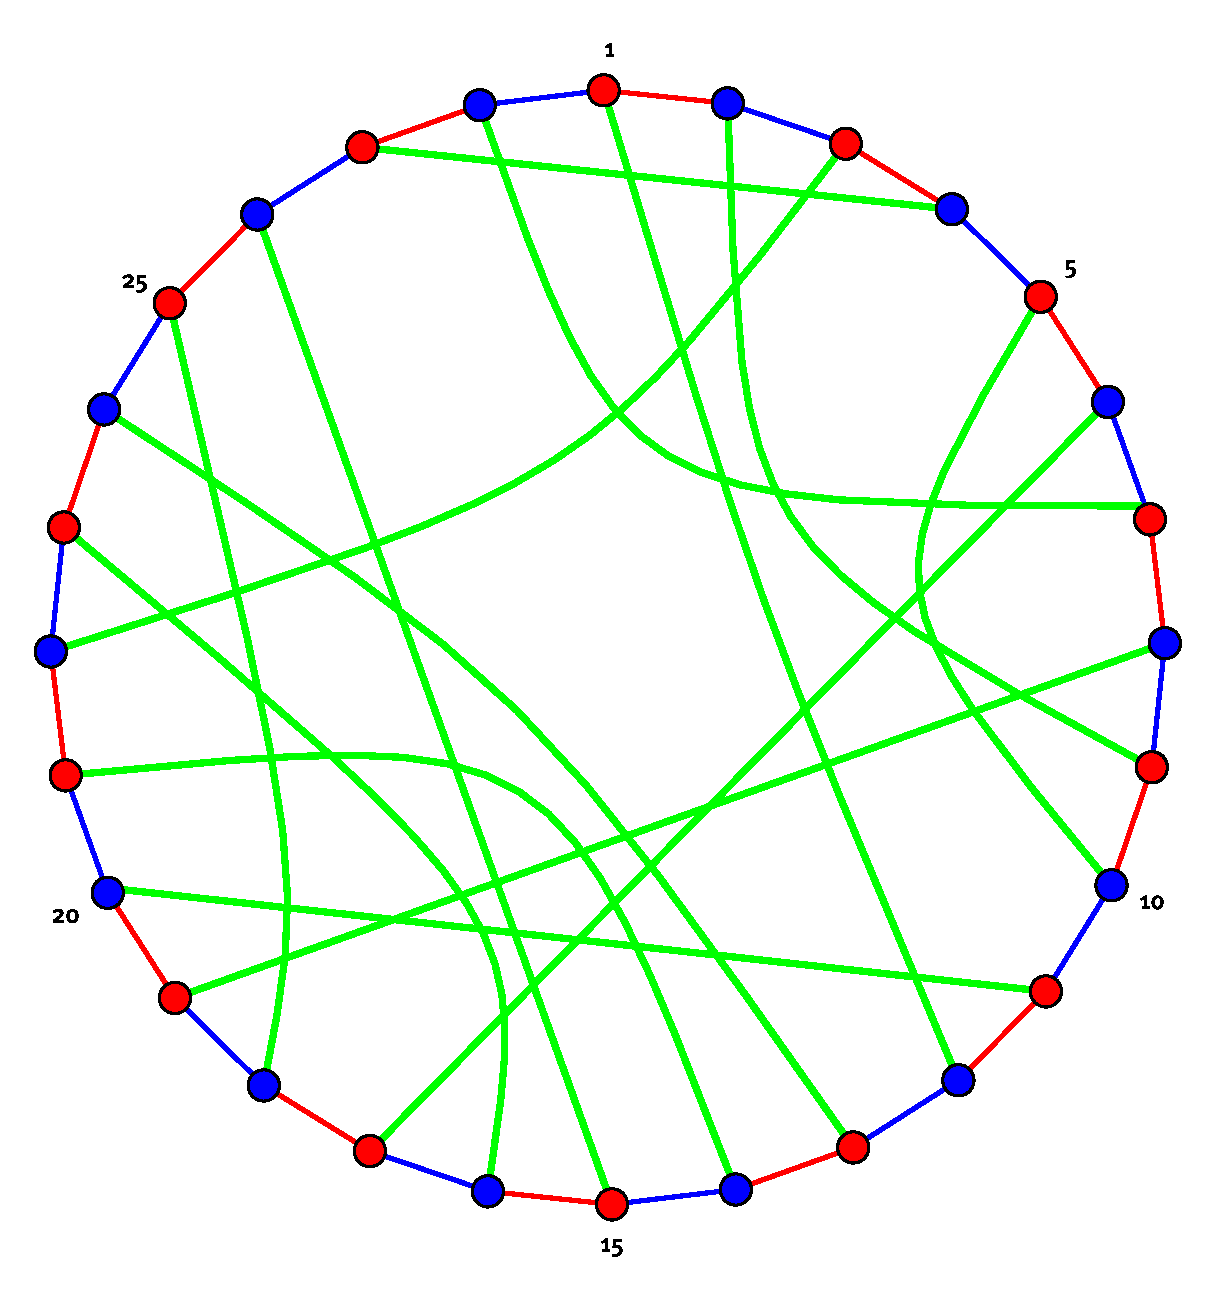
\includegraphics[width=0.95\textwidth]{figures/two_cycles.pdf}

\caption[Smallest bipartite counterexample with three pages]{Smallest bipartite counterexample with three pages containing perfect disjoint matchings where two of the matchings form a cycle.}
\label{figure:two_cycles}
\end{figure}

\paragraph{No restrictions}

If we abandon the restriction that two of the matchings form a cycle, we can proceed similarly. 
Without loss of generality the first matching connects every even vertex to the following odd
vertex. Then the odd and even vertices form the bipartition. The remaining two matchings
can then be filled in by backtracking and adding edges between vertices with different parity. By exchanging
the second and third matching and rotating we can again impose the restriction that~$\mu(0)$
in the second matching is the maximal value of~$\mu(\cdot)$ in both the second and the third matching.

The search space is significantly larger since we abandoned the restriction that two
matchings form a cycle. Thus, we were only able to check for counterexamples up to order~18, which already took a week on the available computing hardware ($4\times12$-Core AMD Opteron 6172, 2.1 GHz, 256 GB RAM). %For 20~vertices
%the program needed too long (TODO, ...). 

We did not find any counterexample with~$\leq 18$ vertices.
That is, we can only conclude that \probThreeMatching
has a smallest bipartite counterexample with at least 20~vertices and at most 28~vertices.

\paragraph{Outlook}

It is, therefore, a sensible extension of this work to implement a
more efficient searcher or just use more computing power to get the
smallest counterexample of \probThreeMatching. 

Also, the special case \probThreeMatching may already be \NP-complete.
It may be possible
to  disprove this by getting a simple decision criterion 
from the structure of the counterexample in \myref{figure:two_cycles}.
Inversely, the example may also provide a clue on how to prove the \NP-hardness. This
direction seems to be quite difficult since we do not really understand why this example is a counterexample.
\section{\PQ-tree on the Vertices}
\label{section:trees}

\noindent 

Besides demanding that pages have a special structure, as we have
done in the preceding sections, we may
restrict the order of the vertices to a subset
of the symmetric group~$S_n$ that we can, hopefully, work with more easily. 

Angelini et.\,al.~\cite{angelini11} showed that \SEFECON~(see page~\pageref{prob:sefecon}) can be reduced to a 2-page embedding problem where the vertex order comes from a \PT-tree.

For this reason it is useful to restrict the permutations with \PQ-trees. That is, we do
the very opposite of \myref{section:connected} and start with a \PQ-tree
instead of getting a tree that represents the possible book embeddings.

\begin{figure}[\placement]\centering
    \includegraphics{figures/t_pq-all}
    \caption[\PQ-tree that represents all permutations]{A \PQ-tree that represents all permutations of $\range{n}$.}
    \label{figure:pq-all}
\end{figure}

A general~\PQ-tree does not really help
since the \PQ-tree in \myref{figure:pq-all} (a single \PT-node) represents all permutations of $\range{n}$,
\ie the problem does not get easier.

Thus, we have to narrow down the possible permutations even more. In this section we only consider
\Q-trees and show that \probQTree, which is \probBook restricted to~\Q-trees,
can be solved in quadratic time. In order to do this, we provide a reduction of the problem to~\probTwoSat, the problem of checking a 2-CNF formula for satisfiability. 
The \probTwoSat problem is solvable in linear time as first shown by Krom~\cite{Krom67}.

\newProb{\probQTree}{A \probBook instance $I$ with vertices $V$ and a \Q-tree~$T$ with leaves~$V$.}{Is there a total order $<\,\in \pi(T)$ solving $I$?}
\newProb{\probPTree}{A \probBook instance $I$ with vertices $V$ and a \PT-tree~$T$ with leaves~$V$.}{Is there a total order $<\,\in \pi(T)$ solving $I$?}
\newProb{\probTwoSat}{A 2-\CNF Boolean formula \bool{f}.}{Is~\bool{f} satisfiable?}

\Q-Trees are exactly the wrong type of trees
compared to the reformulation of the \SEFECON problem by Angelini et.\,al.~\cite{angelini11} since \Q-nodes vastly restrict the possible
permutations and are significantly easier to handle than \PT~nodes. This
section, therefore, only solves \SEFECON if the \PT-tree of the equivalent \probPTree instance is also a \Q-tree, \ie if the \PT-tree is a binary tree.

We first investigate what possible configurations of the leaves the book constraints 
lead to when we take the \Q-tree~$T$ into account. Then we show how these configurations
can be expressed with a 2-\CNF formula.

\paragraph{Possible configurations resulting from a book constraint}

\begin{figure}[\placement]\centering
    \includegraphics{figures/t_topo1}
    \caption[Topologies of four leaves]{The possible topologies of four leaves $a, b, c, d$ in a tree.}
    \label{figure:topo1}
\end{figure}


We first show that the book embedding restrictions for two edges $\{a, b\}$ and $\{c, d\}$
can be translated directly to restrictions on the $Q$-tree.
Before we start with this translation, however, we list some conventions. The \Q-tree is called $T$ and has leaves~$V$. Furthermore, let $t(M)$ be the smallest subtree of~$T$ containing~$M$ and let~$r(M)$ be its root for any~$M \subseteq V$.
Also remember that we assumed  in \myref{section:total-ordering} that any two edges we consider the book constraint for are independent.

%Consider the tree~$t(M)$ for~$M := \{a, b, c, d\}$.

We want to distinguish cases based on which two leaves in~$M := \{a, b, c, d\}$ can be separated from the others. These possible \emph{topologies of $M$ in~$T$} are depicted in \myref{figure:topo1}.
For example, we have~$ab||cd$ if there is an edge~$e \in E(T)$ such that $a$ and~$b$ are
in one component of~$T \setminus e$ while $c$ and~$d$ are in the other component, \ie
$a$ and~$b$ can be separated from $c$ and~$d$.
The topologies for $ac||bd$ and~$ad||bc$ are defined analogously. If no two vertices in~$M$ can be separated from the other
two (all pairs of vertices in~$M$ have the same lowest common ancestor) we say that the topology~$abcd$ occurs. 

%Thus, $t(M)$ has one of the trees in \myref{figure:topo1} as a
%topological minor, \ie the leaves $a$, $b$, $c$ and $d$ can appear
%in only a small number topological configurations. (Note that we do not take into consideration that the tree is rooted and ordered.) We call these configurations ``topologies'' below.

Depending on which of the topologies occurs, we can map the constraint from \myref{lemma:constraints} to a Boolean formula on the order~$<$ of the vertices~$V$.

\paragraph{Case 1: ab||cd}

Since $\{a, b\}$ and $\{c, d\}$ are in disjoint subtrees and the vertices of
a subtree are consecutive in every permutation $\pi(T)$, all tree orders
fulfil the book constraint. Thus, the constraint is mapped to the Boolean expression \bool{true}.

\paragraph{Case 2: ac||bd}

\begin{figure}\centering
    \includegraphics[scale=.9]{figures/t_order_ab_cd}
    \caption[Trees for $ac||bd$]{The possible trees corresponding to $ac||bd$.}
    \label{figure:order_ab_cd}
\end{figure}
\begin{figure}\centering
    \includegraphics[width=\textwidth]{figures/t_topo_ac_bd}
    \caption[Outside 1 tree orders]{The tree orders for the case outside 1.}
    \label{figure:topo_ac_bd}
\end{figure}
\begin{figure}\centering
    \includegraphics[width=\textwidth]{figures/t_topo_b_ac_d}
    \caption[Inside 1 tree orders]{The tree orders for the case inside 1.}
    \label{figure:topo_b_ac_d}
\end{figure}

In this case we search through the possible trees to determine the resulting
\probTwoSat formula. To do this systematically, we have to take into account that~$T$ is ordered and rooted and determine what the tree can look like. 

Thus, we further split this case into sub-cases based on whether the vertices $a$ and~$c$ are between $b$ and~$d$ (inside), $b$ and~$d$ are between $a$ and~$c$ (inside) or no two vertices in~$M$ are between the vertices they are separated from (outside). Note that $a$ and~$c$ are between $b$ and~$d$
for all orders in~$\pi(T)$ if they are between $b$ and~$d$ for one order in~$\pi(T)$ since~$T$
is a \Q-tree.

In the outside case, the
possible permutations also depend on how the roots of the subtrees $t(a, c)$ and $t(b, d)$ are related,
\ie whether one appears as a child of the other. The possible tree structures are depicted
in \myref{figure:order_ab_cd}.  
%We especially need not fix any portion of the order.

For each tree, we can exhaustively search through the orders of the leaves~$M$ the tree permits. For the 
case outside~1 these orders are portrayed in \myref{figure:topo_ac_bd}. We observe that the
valid orders are exactly the orders with $a < c \Leftrightarrow d < b$. The other two outside
cases can be handled similarly. Both of them again yield $a < c \Leftrightarrow d < b$.

For the inside cases we do the same. The possible orders of the case inside~1 are depicted in \myref{figure:topo_b_ac_d}. We can infer the
inverse $a < c \Leftrightarrow b < d$ for both inside cases. 

\paragraph{Case 3: ad||bc}

As in case~2, we either get $a < d \Leftrightarrow b < c$ or
$a < d \Leftrightarrow c < b$.

\paragraph{Case 4: abcd}

Let~$r$ be the common root $r(a, b, c, d)$ of $M := \{a, b, c, d\}$. The tree~$T$
represents two permutations of $M$ since the children of the \Q-node~$r$ can
only be reversed. If the book constraint is valid in a permutation of~$M$, it is also valid in the
mirror image of the permutation. Therefore, the book constraint may be valid in none or both of the two possible permutations. That is, we get either \bool{true} or
\bool{false} as constraint.

\paragraph{Mapping \probBook to \probTwoSat}

We now show how the resulting Boolean expressions can be mapped to \probTwoSat formulae.
To do so we fix a reference orientation of the inner nodes of~$T$.
For each $\pi \in \pi(T)$ and every inner node $v$ in $T$, we can say whether
we got $\pi$ as a permutation in~$\pi(T)$ by giving~$v$ the reference orientation or not.
Introduce a Boolean variable $o_v$ that stands for~$v$ being in reference orientation.

By the construction above, a book constraint for two edges yields one of the following Boolean expressions dependent on the structure of~$T$.

\begin{enumerate}
  \item A trivial expression \bool{true} or \bool{false}. (from cases~1 and~4)
  \item A fixed order of two leaves $v$ and~$w$ which is the same
  as fixing the order of their root~$r := r(v, w)$. Thus, we get
  $o_r$ or $\lnot o_r$. (from case~4)
  \item A connection between the orders of the leaves $a$, $b$ and $c$, $d$
  that are located in disjoint subtrees. This is the same as tying the
  orders of the roots $r := r(a, b)$ and $s := r(c, d)$ together.
  We get either $o_r \Leftrightarrow o_s \equiv (\lnot o_r \lor o_s) \land (\lnot o_s \lor o_r)$
  or $o_r \Leftrightarrow \lnot o_s \equiv (\lnot o_r \lor \lnot o_s) \land (o_s \lor o_r)$. (from cases~2 and~3)
\end{enumerate}

Thus, we can reduce \probQTree to determining whether a set of 2-\CNF expressions
is consistent with a \Q-tree structure. But since the inner nodes of a \Q-tree can be flipped completely independently of each other, the consistency with the \Q-tree structure does not
impose any extra restrictions. That is, \probQTree can be mapped to checking
a \probTwoSat formula for consistency (satisfiability).


%\newProb{\probQTreeSat}{A \Q-tree $T$ and a 2-\CNF expression $m$ on $\{o_v\colon \text{$v$ 
%is inner node of $T$}\}$ with $o_v$~signifying that the node~$v$ is ordered as in the initial tree.}{Is there a permutation in~$\pi(T)$ where~$m$ is satisfied?}

We now see how the reduction from \probQTree to \probTwoSat above can be 
implemented in qua\-dratic time.

\begin{lemma}
\label{lemma:q-tree-redux}
\probQTree can be reduced to \probTwoSat in quadratic time.
%A $\probQTree$~instance  can be reduced
%to a $\probTwoSat$ instance in $\OO\bigl(|T| + |E_1|^2 + \dotsb + |E_k|^2\bigr)$~time.
\end{lemma}
\begin{myproof}
Let $\bigl((V, E_1),\dotsc, (V, E_k), T\bigr)$ be an instance of $\probQTree$.
We can map the book constraints for each pair $e_1, e_2 \in E_i$ of edges for all
$i \in \range{k}$ to a 2-\CNF formula with the construction above.

Let's investigate how this can be done efficiently. Our goal is
to map each book constraint resulting from a pair of edges to a 2-\CNF formula in constant
time after a linear time precomputation. 

We assume $V = \range{n}$ and that each inner node of the tree~$T$ 
contains a pointer to its parent and an (ordered) list of its children.
Furthermore, let~$r$ be the root of~$T$.

%\begin{Ualgorithm}[\placement]
%\caption{Class for rooted, ordered trees}\label{alg:tree}
%\DontPrintSemicolon
%
%\SetKwFor{Class}{class}{}
%
%\SetKwFunction{Tree}{Tree}
%\SetKwFunction{PTree}{Pointer to Tree}
%\SetKwFunction{VTree}{Vector of pointers to Tree}
%\SetKwFunction{MyInt}{Integer}
%
%\Class{\Tree}{parent: \PTree\;children: \VTree}
%\end{Ualgorithm}

To determine the topology of a quadruple of leaves, we need to know
the lowest common ancestor of certain pairs of nodes and their initial order.

The first problem has been studied extensively. Harel and Tarjan~\cite{Harel84} showed
the surprising result that lowest common ancestor queries can be answered in constant
time after a linear time precomputation, although their algorithm was too complicated to be implemented
effectively. Farach and Colton~\cite{Farach00} presented a far simpler variant of this
algorithm that is used in practice. We assume in the following that the precomputation has 
been done and that \algoFont{LCA($x$, $y$)} gives the lowest common ancestor of~$x$ and~$y$ in~$\OO(1)$ time.

For the second problem, we can precompute the index array~\algoFont{idx} of~$V$ that maps each
leaf~$V$ to its index in the reference orientation of~$T$. This can be accomplished in linear time by a simple depth-first search. 

%At each step,
%we know the index the leaves in the current subtree start with. We recurse on the children
%of the current node in order and update the starting index accordingly. When we arrive at a
%leaf, we know that its index is the current starting index, which is given as a parameter. The initial
%call is~\algoFont{ComputeIndex$(r, 1)$}.
%
%\begin{Ualgorithm}[\placement]
%\caption[Computing the index array]{Computing the index array: \algoFont{ComputeIndex}}\label{alg:index}
%
%\SetKwFunction{Tree}{Tree}
%\SetKwFunction{ComputeIndex}{ComputeIndex}
%\SetKwFunction{size}{size}
%\SetKwFunction{content}{idx}
%\SetKwFunction{children}{children}
%
%\SetKwData{T}{T}
%\SetKwData{firstIdx}{s}
%\SetKwData{lastIdx}{e}
%\SetKwData{idx}{idx}
%\SetKwData{mycnt}{i}
%
%\KwIn{Tree $T$, starting index $s$}
%\KwOut{Ending index $e$}
%
%\BlankLine
%\tcp{Is $T$ leaf?}
%\If{$\T.\children.\size = 0$}{
%$\lastIdx \leftarrow \firstIdx$ \;
%$\idx[\T.\content] \leftarrow \firstIdx$
%}
%\Else {
%	\tcp{Recurse and update indexes}
%	\For{$\mycnt \leftarrow 1$ to $\T.\children.\size$}{
%		$\firstIdx \leftarrow \ComputeIndex(\T[\mycnt], \firstIdx) + 1$
%	}
%}
%\end{Ualgorithm}

Before we begin with the actual translation, we need another helper function \algoFont{Leaf-Order($a$,$b$)} that translates a statement
of the form~$a < b$ for leaves $a, b \in V$ into a literal on the variable~$o_r$ 
where $r = \algoFont{LCA}(a, b)$. If $\algoFont{idx[a]} < \algoFont{idx[b]}$, then~$r$ has reference orientation and the result is~$o_r$. Otherwise, the result is~$\lnot o_r$. This decision can obviously
can be made in $\OO(1)$~time.

%\begin{Ualgorithm}[\placement]
%\caption[Literal for leaf order]{A literal for a given leaf order: $\algoFont{Leaf-Order}$}\label{alg:lca}
%
%\KwIn{Leaves $a, b \in V$}
%\KwOut{A Boolean formula representing $a < b$}
%
%\SetKwFunction{LCA}{LCA}
%
%\SetKwData{firstPar}{a}
%\SetKwData{secondPar}{b}
%\SetKwData{idx}{idx}
%
%\BlankLine
%$r \leftarrow \LCA(\firstPar, \secondPar)$ \;
%\If{$\idx[\firstPar] < \idx[\secondPar]$}{
%	\KwRet $o_r$
%}
%\Else{
%	\KwRet $\lnot o_r$
%}
%\end{Ualgorithm}

We now have everything we need to translate book constraints into
Boolean formulae. The direct formalisation of the construction
above is given in \myref{alg:translate}. It returns
a Boolean formula for a pair of edges $\{a, b\}$ and~$\{c, d\}$
in~$\OO(1)$. Note that we can test whether the order~\algoFont{idx} fulfils
the book constraint in line~9 in~$\OO(1)$ time since only the relative
order of $a$, $b$, $c$ and $d$ is relevant.

In the algorithm, the Boolean formulae are not given in conjunctive normal
form for the sake of clarity. If we want \CNF~formulae, we can statically replace
the Boolean formulae in \myref{alg:translate} by their \CNF~equivalents.


\SetAlFnt{\footnotesize\sffamily}
\begin{Ualgorithm}[\placement]
\caption[Translating the book constraint in $\OO(1)$]{Translating the book constraint in $\OO(1)$ }
\label{alg:translate}

\SetKwFunction{LCA}{LCA}
\SetKwFunction{LeafOrder}{Leaf-Order}

\SetKwData{pa}{a}
\SetKwData{pb}{b}
\SetKwData{pc}{c}
\SetKwData{pd}{d}
\SetKwData{idx}{idx}

\KwIn{Two edges $\{\pa, \pb\}$ and $\{\pc, \pd\}$}
\KwOut{A Boolean formula representing the book constraint for the two edges}

\BlankLine

\tcp{Independent edges?}
\If{$|\{\pa, \pb, \pc, \pd\}| = 4$}{
	$r_1 \leftarrow \LCA(\pa, \pb)$ \;
    $r_2 \leftarrow \LCA(\pa, \pc)$ \;
	$r_3 \leftarrow \LCA(\pa, \pd)$ \;
	$r_4 \leftarrow \LCA(\pb, \pc)$ \;
	$r_5 \leftarrow \LCA(\pb, \pd)$ \;
	$r_6 \leftarrow \LCA(\pc, \pd)$ \;
	\If{all~$r_i$ are the same for~$i \in \range{6}$}{
		\tcp{$abcd$}
%		$x \leftarrow \text{leaf with smallest \idx among \pa, \pb, \pc and \pd}$ \;
%		$y \leftarrow \text{leaf with largest \idx among \pa, \pb, \pc and \pd}$ \;
		\If{Order \idx fulfils book constraint}{
			\KwRet $true$
		}
		\Else{
			\KwRet $false$
		}
	} \ElseIf{$\LCA(r_2, r_5)$ is not equal to $r_2$ or $r_5$}{
		\tcp{$ac||bd$}
		\If{$\idx[\pa]$ between $\idx[\pb]$ and $\idx[\pd]$}{
			\KwRet $\LeafOrder(\pa, \pc) \Leftrightarrow \LeafOrder(\pb, \pd)$
		}
		\Else {
			\KwRet $\LeafOrder(\pa, \pc) \Leftrightarrow \LeafOrder(\pd, \pb)$
		}
	} \ElseIf{$\LCA(r_3, r_4)$ is not equal to $r_3$ or $r_4$}{
	    \tcp{$ad||bc$}
	    \If{$\idx[\pa]$ between $\idx[\pb]$ and $\idx[\pc]$}{
			\KwRet $\LeafOrder(\pa, \pd) \Leftrightarrow \LeafOrder(\pb, \pc)$
		}
		\Else {
			\KwRet $\LeafOrder(\pa, \pd) \Leftrightarrow \LeafOrder(\pc, \pb)$
		}
	} \Else {
	    \tcp{$ab||cd$}
		\KwRet $true$
	}
}
\Else{
	\KwRet $true$
}
\end{Ualgorithm}

All in all, we need~$\OO\bigl(|T|\bigr)$ time for the precomputation and
$\OO(1)$~time for each of the~$\OO\bigl(|E_1|^2+\dotsb+|E_k|^2\bigr)$ book constraints.
Thus, the reduction to \probQTreeSat takes $\OO\bigl(|T| + |E_1|^2 + \dotsb + |E_k|^2\bigr)$~time.\qedhere
%We need to determine the topological structure of each of the
%$|E_1|^2 + \cdots + |E_n|^2$ edge pairs $e_1$ and $e_2$. This
%can be done in~$\OO(|T|)$ by following a path from a vertex of $e_1$ to the root
%if we have a bit-field of length $\OO(|V|)$ for each inner node $v$~of~$T$ from which we
%can determine, whether a leaf is contained in the subtree rooted at~$v$. The bit-field
%can be recursively precomputed in time $\OO(|T|^2|V|)$.

%Thus, the reduction to \probQTreeSat takes $\OO(|T|\cdot(|E_1|^2 + \cdots + |E_n|^2 + |V||T|))$~time
\end{myproof}

%The problem~\probQTreeSat is clearly efficiently solvable.

%\begin{lemma}
%An instance~$(T, m)$ of \probQTreeSat can be solved in $\OO\bigl(|m|\bigr)$.
%\end{lemma}
%\begin{myproof}
%The inner nodes of~$T$ can be flipped completely independently of each other,
%\ie there are no constraints on the~$o_v$ except the ones given in~$m$.
%Since~$m$ is a 2-\CNF expression, checking it for consistency (satisfiability)
%can be done in $\OO\bigl(|m|\bigr)$ as first shown by Krom~\cite{Krom67}.
%\end{myproof}

Since \probTwoSat is solvable in linear time, we conclude that \probQTree can be solved in quadratic time.

\begin{theorem}
\label{theorem:q-tree-book}
\probQTree can be solved in quadratic time.
\end{theorem}
\begin{myproof}
Let $\bigl((V, E_1),\dotsc, (V, E_k), T\bigr)$ be an instance of $\probQTree$.
We saw that the reduction to \probTwoSat takes $\OO\bigl(|T| + |E_1|^2 + \dotsb + |E_k|^2\bigr)$ time
in \myref{lemma:q-tree-redux}. For each pair of edges $e_1, e_2 \in E_i$ where $i \in \range{n}$ we get a 2-\CNF expression of length $\OO(1)$. Since \probTwoSat is solvable in linear
time as first shown by Krom~\cite{Krom67}, we, therefore, need $\OO\bigl(|E_1|^2 + \dotsb + |E_n|^2\bigr)$~time to solve the resulting \probTwoSat problem.
Altogether, we need $\OO\bigl(|T| + |E_1|^2 + \dotsb + |E_k|^2\bigr)$ time.
\end{myproof}

We have assumed $|E_i| \le 2|V|-3$ for all~$i \in \range{k}$ at the
start of \myref{ch:preliminaries} since the pages
have to be outerplanar to be embeddable. Furthermore, the \Q-tree 
has fewer inner nodes than its number of leaves~$|V|$ since each inner node
has at least two children.
That is, we can rewrite the time as
$\OO\bigl(|T| + |E_1|^2 + \dotsb + |E_k|^2\bigr) = \OO\bigl(|V| + k(2|V|-3)^2\bigr) = \OO\bigl(k|V|^2\bigr)$.

\paragraph{Outlook}

So book embedding is solvable in quadratic time if we constrain the vertex order by a \Q-tree. But what if we have a \PT-tree as in the
reformulation of \SEFECON? We have already seen in \myref{figure:pq-all} that this
restriction cannot make the problem simpler than the general book embedding problem. Furthermore, we cannot directly generalise our construction since the answer to ``What permutation of the children of a \PT-node occurs?'' cannot simply be modelled by a Boolean variable.
%for example, the sub-argument for $ac||bd$ depends on us being able to distinguish between the inside
%and outside cases. If the common root $r := r(a, b, c, d)$ were a \PT-node, the tree would
%allow permutations with $ac$ between~$bd$ and permutations where this is not the case, \ie there are %valid
%orders with $a < c \land b < d$ and ones with $a < c \land d > b$. This means that we cannot simply
%model the book constraint by looking at how~$r$ is flipped.
That is, \probPTree remains an
interesting open problem.
\section{Multiple Spines}\label{section:multi_spine}

In the previous sections we showed how \PQ-trees relate
to book embeddings. On the one hand they can help to solve
the problem for connected graphs on the pages and on the other hand
we can restrict the orders of the vertices with a \PQ-tree, yielding
an interesting modification to book embedding.

\begin{figure}[\placement]\centering
    \includegraphics{figures/t_two_spines}
    \caption[Two-spine drawing]{A two-spine drawing.}
    \label{figure:two_spines}
\end{figure}

We now consider another variation on book embedding which 
will turn out to be a special case of the latter application of \PQ-trees.
It is a generalisation of the 2-page case that uses not just one spine but several parallel
spines~(lines) $S_1$, \dots, $S_k$. In the following considerations we always assume
that $S_i$~is above~$S_{i+1}$ for all $i\in\range{k-1}$.
We want to planarly draw one graph above~$S_1$,
one between~$S_i$ and $S_{i+1}$ for each $i \in \range{k-1}$ and one
below~$S_k$, as depicted in \myref{figure:two_spines} for
two spines. This problem is motivated by \emph{level planarity} which
is the same problem without the \emph{caps}, the graph above~$S_1$ and
the graph below~$S_k$.
The level planarity problem was first introduced by Tomii~et.~al.~\cite{Tomii77}. 
Jünger, Leipert and
Mutzel presented an algorithm that checks for level planarity in linear time~\cite{Junger99}.

In this section we show that the multiple spine problem is equivalent to a 2-page book embedding problem constrained by a special \PT-tree, but do not manage to give an efficient algorithm
it. Still, this reinforces our belief that \probPTree is an interesting problem.

Let the spines always be~$S_i = \SR \times \{-i\}$. We now formally define
the problem. It will turn out to be convenient to formally use directed edges pointing downward for the edges between the spines, but we still understand and draw these edges as undirected edges.

\newProb{\probMul}{Vertex sets~$V_1$, \dots, $V_k$ and
edge sets $E_0 \subseteq \binom{V_1}{2}$, $E_1 \subseteq V_1\times V_2$,
\dots, $E_{k-1} \subseteq V_{k-1} \times V_k$, $E_k \subseteq \binom{V_k}{2}$.}{Is there
a planar drawing of $(V_1 \cup \dotsb \cup V_k, E_0 \cup \dotsb \cup E_k)$ such that
a vertex in~$V_i$ lies on~$S_i$ for all~$i \in \range{k}$, edges do not cross a spine,
the edges in~$E_0$ lie completely above~$S_1$ and the edges in~$E_k$ lie completely below~$S_k$?}

Tomii~et.~al.~\cite{Tomii77} showed that the 2-level planar graphs are exactly the forests
of caterpillars. Recall that a \emph{caterpillar} is a tree all of whose vertices are on
a central path or one edge away from it. Therefore, each of the graphs~$(V_i \cup V_{i+1}, E_i)$ for~$i \in \range{k-1}$ has to be a forest, \ie we find~$|E_i| = |V_i| + |V_{i+1}| - l$ if this
forest has $l$~components. That is, as in the case of page embedding the number of edges is again linear in
the number of vertices. Thus, the size of a \probMul~instance is in~$\OO\bigl(|V_1| + \dotsb + |V_k|\bigr)$.

\begin{figure}[\placement]\centering
    \includegraphics{figures/t_level_order}
    \caption[Level planarity is an ordering problem]{Level planarity only depends on the order of the vertices.}
    \label{figure:level_order}
\end{figure}

From \myref{lemma:constraints} we know that book embedding is essentially an ordering problem.
Similarly, consider two edges $(a_1, b_1)$ and~$(a_2, b_2)$ lying between the same two spines
and investigate how their embeddability depends on the order of their endpoints. If
$a_1$~lies left of~$a_2$ on the upper spine and $b_2$~lies left of~$b_1$ on the lower spine, then any Jordan curve from $a_1$ to~$b_1$ between the spines must intersect with any Jordan curve from $a_2$ to~$b_2$ between the spines by the Jordan curve theorem, \ie there cannot 
be a level embedding with this order. This case is depicted in \myref{figure:level_order}. Similarly,
if $a_2$~lies left of~$a_1$ and $b_1$~lies left of~$b_2$, the edges~$(a_1, b_1)$ and~$(a_2, b_2)$ also
cannot be embedded.

In any other order we can just draw a straight line for both
edges to obtain a valid embedding of the edges. After combining these observations for all pairs
of edges and taking the caps into account, we get a total order formulation of \probMul.
 
\begin{lemma}\label{lemma:multi_spine_total}
Let~$I := (V_1, \dotsc, V_k, E_0, \dotsc, E_k)$ be a \probMul instance. Then~$I$ is solvable
if any only if there is a linear order~$<_i$ on~$V_i$ for each $i \in \range{k}$ such
that the following properties hold. For all~$i \in \{1, \dots, k-1\}$ and pairs of edges~$(a_1, b_1), (a_2, b_2) \in E_i$ the order $a_1 <_i a_2 \land b_2 <_{i+1} b_1$ does not occur. Furthermore,
for $i\in\{0, k\}$ and all $\{a, b\}, \{c, d\} \in E_i$ we must not have $a <_i c <_i b <_i d$.
\end{lemma}

The order constraint for level planarity looks very similar to the book constraint,
just separated into two total orders. Indeed, if we have a \probMul instance we can find a corresponding
book embedding instance.
\begin{figure}\centering
    \includegraphics[width=0.9\textwidth]{figures/t_level_map}
    \caption[\probMul instance to book embedding instance]{A \probMul instance can be transformed into a 2-page book embedding instance
with separated sets of vertices.}
    \label{figure:level_map}
\end{figure}
\vskip1em
\begin{theorem}
Let~$I := (V_1, \dotsc, V_k, E_0, \dotsc, E_k)$ be a \probMul instance. We define
a corresponding 2-page book embedding instance by taking $V := V_1 \cup \dotsb \cup V_k$
as vertices and 
\begin{align*}
\widetilde{E}_1 := \bigcup_{\substack{i \in \{0, \dotsc, k\}\\ i \text{\emph{ even}}}} E_i\\
\widetilde{E}_2 := \bigcup_{\substack{i \in \{0, \dotsc, k\}\\ i \text{\emph{ odd}}}} E_i
\end{align*}
as pages. Then~$I$ is solvable if and only if~$J := (V, \widetilde{E}_1, \widetilde{E}_2)$
has a book embedding where the vertices in each~$V_i$ are consecutive.
\end{theorem}

\begin{myproof}
\begin{itemize}
\item[]
\item[``$\Rightarrow$''] Let~$<_i$ for~$i \in \range{k}$ be total orders forming a valid 
embedding of~$I$. 

Then define~$<$ on~$V$ to be the total order that first lists the
vertices of~$V_1$, then the vertices of~$V_2$, and so on. Get the inner order of the vertices
in~$V_i$ from~$<_i$ if~$i$ is even and from~$<_i$ reversed if~$i$ is odd. This
construction is illustrated in \myref{figure:level_map}.

The order~$<$ is a valid solution of the book embedding problem~$J$:
The edges in distinct edge sets~$E_i$ do not intersect by the construction of~$<$ and the definitions
of $\widetilde{E}_1$ and $\widetilde{E}_2$. Edges in~$E_0$ or~$E_k$ do not intersect since~$<_1$
and~$<_k$ are valid page embeddings for~$(V_1, E_0)$ and~$(V_k, E_k)$, respectively. Now take
two edges~$(a_1, b_1), (a_2, b_2) \in E_i$ for some~$i \in \range{k-1}$. If~$a_1 < a_2 < b_1 < b_2$
occurs, we have~$a_1 <_i a_2\;\land\;b_1 <_{i+1} b_2$, contradicting the validity of
the initial solution of~$I$. Thus, the book constraint for the two edges is fulfilled.
\item[``$\Leftarrow$''] Let~$<$ be a valid book order of~$J$ where
the sets~$V_i$ with~$i \in \range{k}$ are separated. Do the construction above in reverse, \ie
define~$<_i$ to be the restriction of~$<$ to~$V_i$ for all~$i \in \range{k}$. Additionally,
reverse~$<_i$ when~$i$ is odd.

The order~$<_i$ yields a valid embedding for~$I$: The caps already appeared in the book embedding
problem~$J$, \ie they are still valid. If~$a_1 <_i a_2\;\land\;b_2 <_{i+1} b_1$ occurs for some~$(a_1, b_1), (a_2, b_2) \in E_i$ and~$i \in \range{k-1}$, then we must have either~$a_1 < a_2 < b_1 < b_2$,
$a_2 < a_1 < b_2 < b_1$, $b_1 < b_2 < a_2 < a_1$ or~$b_2 < b_1 < a_1 < a_2$. All of these
cases contradict the book constraints.\qedhere
\end{itemize}
\end{myproof}

\paragraph{Outlook}

All in all, we see that \probMul is equivalent to a 2-page book
embedding problem where the vertex sets~$V_i$ with~$i \in \range{k}$ have to be 
separated. This separation can be modelled by a \PT-tree by introducing a \PT-node
connected to the vertices~$V_i$ for all~$i \in \range{k}$ and connecting all 
of these \PT-nodes to a single root. 

Since \probMul is an interesting problem in its own right, this leaves several
distinct possibilities for further results:
\begin{itemize}
\item Provide a polynomial time algorithm for  \probPTree and get an efficient solution of \probMul.
\item Prove the \NP-completeness of \probMul and get the \NP-completeness of \probPTree.
\item Provide a polynomial time algorithm for \probMul and get an efficient algorithm for a special case of \probPTree.
\end{itemize}